\chapter{Sketch It, Make It: Overview}

The primary contribution of this thesis is the set of interaction
techniques implemented in a single design tool called Sketch It, Make
It (SIMI). SIMI is a modeling environment for laser cutter design that
recognizes short sequences of drawn input made with a stylus. Using
only freehand input, SIMI enables a designer to iteratively and
incrementally create precise laser cut models.

I am inspired by the potential of freehand drawing as the basis for
precision modeling for several reasons. Sketching is quick and can be
easily learned. It is simple and modeless: unlike structured editing
software, a designer need not set a pencil's mode to line, circle, or
anything else. I will show that given an appropriate set of
interaction methods, sketched input can provide enough information to
make a precise digital model.

There are several principles that guided SIMI's design and development.

\begin{itemize}
\item \textbf{Democratized design}: Freehand drawing is a skill that
  most people already have. It follows that a tool based on sketch
  based interaction should be usable by a majority of people. For this
  reason I target avocational designers, not professionals. 
\item \textbf{Sketch based}: The user should never feel obliged to set
  down their pen. In the past, many sketch based design tools have
  relied on keyboard input, or used interface widgets that are
  appropriate for mice but are uncomfortable to use with a stylus
  (e.g. hierarchic menus).
\item \textbf{Coherence of interaction techniques is key}: The tool
  presents a set of sketch based interaction techniques that work well
  together. Researchers commonly make toy systems that demonstrate one
  or two novel interaction techniques in isolation (e.g. my own prior
  work on Flow Selection~\cite{johnson-flow-selection}). But a useful
  tool has many individual techniques. The current system implements
  many techniques together to give an example of a way to make them
  work harmoniously.
\item \textbf{Useful and usable}: Last, the system lets people make
  real things in a real domain (namely, laser cut objects). The
  current implementation of the tool is efficient and highly
  responsive. In informal demonstrations, more than one person has
  noted that the system seems more like a commercial product than a
  research system. This is intentional.
\end{itemize}

\section{Rapid Fabrication and Laser Cutting}

Laser cutters are among the more common and affordable fabrication
machines. One can think of a laser cutter as a fast, strong, and
precise automated razor that cuts flat material (paper, wood, plastic,
textiles, etc.). 

% Price information: 
% 2001: 12,900 (ULS 25 watt)
% 2006: 9,995 (ULS 25 watt)
% 2010: 8,500 (ULS 25 watt)
% 2011: 6,850 (ULS 25 watt)
%
%   http://www.rcgroups.com/forums/showthread.php?t=16912 claims that
%   a 25-watt model from Universal Laser systems cost $12,900. Several
%   comments in that thread are in line with that price estimate for
%   home-garage-lab use.
%   http://www.microgeo-usa.com/ProductDetails.asp?ProductCode=universal-laser-VLS2.30
%   currently prices the ULS 25 watt 16x12 unit as costing $6,850.

% http://55-website.com/xo1/ulsinc/english/PDFs/EJ_VL_Article_Reprint.pdf is a press article from 2006 that prices the 25 watt laser at 10,000
\begin{figure}[b] %  figure placement: here, top, bottom, or page
   \centering
   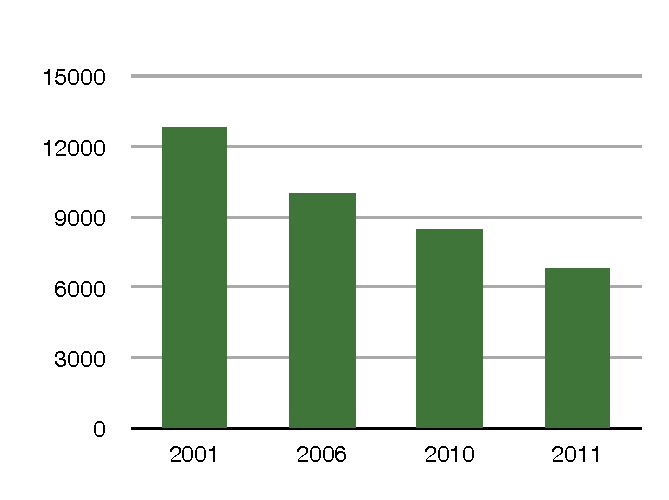
\includegraphics[width=3in]{img/prices.pdf} 
   \caption[Declining laser cutter prices]{Declining prices of Universal Laser Systems 25-Watt 16x12
     inch laser cutter (US Dollars).}
   \label{fig:prices}
\end{figure}


The price of laser cutters is quickly declining, making it possible
that more people have access to them. Figure~\ref{fig:prices} shows
prices for a comparable~25-Watt,~16''x12'' laser cutter model from
Universal Laser Systems (these values were found on hobbyist web
forums). While these data may not be exact, they do show the price of
desktop laser cutting machines has been cut by almost half in the past
ten years. While still out of reach for most people to afford, they
are becoming inexpensive enough for schools and hacker spaces to own.

Laser cut designs are composed of parts cut from solid, flat material
and assembled in various ways: laminated, notched, bolted together,
\textit{etc}. Various materials require different laser speed and
intensity settings to achieve a quality cut. The designe uses a
software application to specify part shapes for laser cutting. The
software outputs vector graphics called a ``cut file'' that defines
these shapes. As most joints have small margins of error, lengths,
angles, and relative position must be specified precisely so that
parts fit together properly.

Tools for designing laser cut objects must allow users to precisely
specify dimensions. Like a physical saw, the laser leaves a gap in its
wake, called a \textit{kerf}, (between 0.2mm and 0.5mm on a 40 watt
cutter). This is an important consideration when designing facets
whose tolerances are small with respect to kerf. A notch joint, for
example, is ineffective if it is 0.1 mm too large or small.


\section{Motivating Scenario: Pictureframe Holder}

\begin{figure}
  \centering
  \begin{subfigure}[b]{0.45\textwidth}
    \centering
    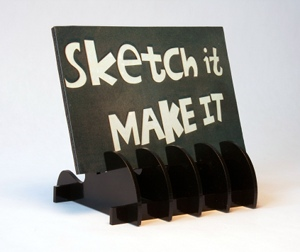
\includegraphics[width=\textwidth]{img/simi-stand-withpic.jpg}
    \caption{} % force the (a) to show up
    \label{fig:example-1}
  \end{subfigure}
  \begin{subfigure}[b]{0.45\textwidth}
    \centering
    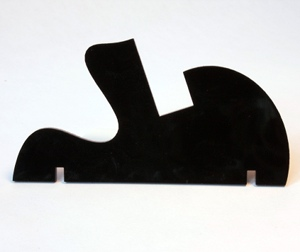
\includegraphics[width=\textwidth]{img/simi-stand-part.jpg}
    \caption{} % force the (b) to show up
    \label{fig:example-2}
  \end{subfigure}
  \caption[Picture Frame Stand]{A picture stand (\subref{fig:example-1})
    drawn and fabricated using SIMI. A single copy of the primary part
    is shown in (\subref{fig:example-2}). }
  \label{fig:simi-example}
\end{figure}


To introduce Sketch It, Make It I will explain how it could be used to
make the picture stand shown in Figure~\ref{fig:simi-example}. This
narrative helps explain the overall user experience while exposing
technical aspects (which are discussed in much greater detail in the
following chapter).

We begin with the idea of a stand with two horizontal rails as a base
and a five-part vertical support structure, joined with notches. Using
SIMI on a tablet device like the Wacom Cintiq shown in
Figure~\ref{fig:simi-intro}, we first draw the rough profile of the
vertical support piece using curved and straight segments. After a
brief period of inactivity, SIMI captures our drawing, straightening
lines, smoothing curves, and connecting curved and straight
segments. We may optionally press a button with our non-dominant hand
to ask SIMI to do this immediately. If we make a mistake (or if we
change our mind), we can recover quickly by scratching out the
unwanted ink, or use an Undo gesture.

After sketching the rough outlines of our two parts, we begin to
refine the design and make it precise.  We square the corners by
drawing right-angle braces (Figure~\ref{fig:motivating}a).  Now as we
adjust the shapes of the two parts by selecting and dragging endpoints
and re-shaping curves, SIMI maintains the right-angle constraints
we've established.
 
Next, we add notches to the two parts for the joints. We draw five
small notches on the base rail. For each notch we draw three lines
inside the outline of the part, and then use the erase gesture to
remove the residual outline segment (Figure~\ref{fig:motivating}b).
Then we indicate that both sides of the notch are to be the same
length: We draw tick marks on each segment, and right-angle braces to
keep the notch perpendicular to the edge of the part. The notches must
have exactly the right dimensions: too wide, the top parts will
wobble; too narrow and they will not fit. We size the notch by
overtracing its segments and entering fixed dimensions
(Figure~\ref{fig:motivating}c).
 
We drag the base part (twice) and the support part (five times) to
SIMI's cut file area to prepare a PDF file for cutting, and then send
it to the laser cutter.  Finally we assemble the cut parts to make the
picture stand in Figure~\ref{fig:simi-example}.

\begin{figure}
  \centering
  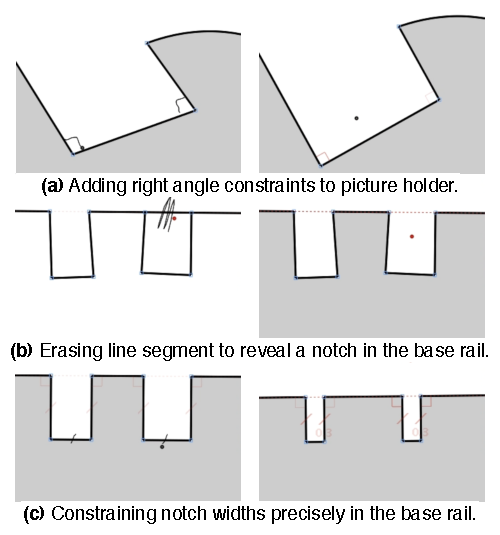
\includegraphics{img/motivating-example.pdf}
  \caption[Interaction steps to a picture frame]{Key steps taken when
    making the picture stand.}
  \label{fig:motivating}
\end{figure}


\section{Technical Challenges Met By SIMI}

The above section describes the user's needs, and how the user
interacts with the system. This section summarizes several categories
of technical challenges the system has to meet in order to support
those user needs. These categories are printed in bold text. Most of
the following topics are described in great detail in the next
chapter.

A fundamental task is \textbf{ink parsing}. While the pen is down, the
system looks for erase gestures. When the user lifts the pen,
non-erase gestures are parsed for corners, and sections of ink are
identified as primitive sub-shapes like lines, curves, and so forth.

SIMI must be able to dependably \textbf{recognize user input}.
Because input is often made quickly and inaccurately, occasional
recognition errors can not be avoided. There are several kinds of
recognized elements. Input might be linework that specifies the
model's geometry. Or, input might be identified as a gesture that
edits the model by removing ink or adding constraints. Last, input
might be as part of a multi-stroke phrase that controls the modeling
environment (e.g. undo/redo, zooming, or panning).

There is one recognizer per recognizable pattern. Each recognizer has
access to the model state, but they do not communicate directly with
each other. Inevitably more than one recognizer will signal a positive
result, so it is necessary for SIMI to \textbf{disambiguate}
contending recognition results. For example, the user may draw two
short strokes that are recognized as both a right angle symbol and a
same-length gesture. To resolve this ambiguity, SIMI uses a series of
tests that involve context (e.g. if the input is correctly positioned
in a corner or not) as well as static precedence rules that defer to
the interpretation that causes the least trouble in the event it is
wrong.

\missingfigure{Need a figure of the recognizer architecture. Several
  kinds of recognizers (linework, dynamic, pen-up, and delayed), and
  two different opportunities to disambiguate contending input}

The user's work is stored as a \textbf{data model} consisting of
points, segments (e.g. line, arc), and high-level constraints
(e.g. right angle, same length). SIMI lets the user edit the model to
create, merge, or erase these elements. The \textbf{constraint engine}
is closely associated with the data model. This lets the designer
indicate geometric rules that the system will try to maintains, even
as the user edits the model. SIMI's constraint engine is an iterative,
numerical solver using a relaxation method in the tradition of
Sketchpad~\cite{sutherland-sketchpad}.

When it is time for the user's work to be given to a laser cutter, the
designer asks SIMI to \textbf{generate a cutfile}. This is a 2D vector
graphics file specifying geometry of cutouts. The current
implementation is a rather simplistic ``typewriter'' algorithm---it
uses the bounding box of each cutout, placing one next to the other
from left to right, and moving to the next ``line'' when placing a
piece would extend beyond the material bounds.

\section{Coherent Sketch Based Interaction}

TODO...

From the user's perspective, SIMI gives a new kind of experience
because it:

\begin{itemize}
\item Is ``modeless''. Should describe the mode problem, why
  overcoming it is such an important thing, and why it is especially
  pertinent to sketch-based interaction. (because if we have modes, we
  are essentially on slippery-slope to MouseCAD)
\item Is incremental, rather than one-big-batch style recognition that
  is so popular
\item Uses ``more natural'' input. The pen is easier to manipulate
  than the mouse. Naturalness is a common term but is ultimately
  meaningless because all design tools are artificial. Could say it
  has less cognitive and ergonomic demands than modal, mouse-based
  tools
\item From a domain perspective it is not over featured, so it is
  clear how to proceed.
\end{itemize}

\section{Implementation Architecture}

TODO...

Here try to give a concise description of the system architecture. The
next chapter is about individual interaction techniques, but it
doesn't talk about how they are coordinated. So I should do that here,
and hand-wave about how individual techniques work.
